\graphicspath{ {./images/} }
\chapter{背景}
\label{c:background}


\section{區塊鏈}

在區塊鏈網路中的每一個全節點(full node)都會維護一份完整的賬本,
賬本記錄了過往所有區塊中的交易,由此我們能夠知曉交易發生的時間點、交易的付款人收款人、交易的金額,
付款人得以向付款人證明自己確實已經付款。

區塊鏈網路中,賬本的更新以區塊為單位,
當一個礦工節點蒐集交易並挖掘出一個區塊後,
會將它廣播到網路上,收到區塊的節點必須驗證後決定是否接收,
若接收,賬本的內容就得到更新。

根據收付款的方式,區塊鏈貨幣可分為類似零錢式的 UTXO 系統,
以及類似銀行賬戶式的賬戶系統,
在本論文中,只關注基於賬戶的區塊鏈系統,忽略 UTXO 的區塊鏈系統。

\subsection{區塊驗證}

在支援智能合約的賬戶系統中,對於區塊中的一般交易,
節點必須知道付款人是否有足夠的餘額;
若涉及智能合約,節點需要獲取合約程式碼以及合約當前的狀態,
才能夠執行合約。

我們可以用一個鍵值對來表示賬戶系統在驗證交易時所需要儲存的資訊:

\[state = f: address\to account \]

給一個地址,我們能得到對應賬戶的資訊,可能是餘額,也可能是智能合約的狀態。

若要儘速完成這些工作,節點必須快速地檢索交易,因此,
一個一個區塊地尋找、計算出賬戶資訊是不切實際的, 
通常節點會內置一個資料庫,並利用資料庫的索引來高速完成查詢工作。

\subsection{狀態儲存的問題}

區塊鏈的狀態儲存方式造成了兩個危害:

\begin{enumerate}
  \item 佔用硬碟空間大
  \item 驗證交易時需要硬碟隨機存取
\end{enumerate}

\subsubsection{佔用硬碟空間大}

永遠增長的區塊已經對節點維護者造成負擔,比特幣與以太坊佔用的空間都已經超過 200 GB ,
如果在 AWS 上租用機器來運行以太坊節點,每個月需花費 50 - 70 美金,
這個成本如果降不下來,慈善節點的數量勢必會不斷下滑,
根據 \url{https://ethernodes.org/} 的資訊,2018 年仍有將近兩萬個節點,2020 年已經下降到七千。

另外一個問題是,以太坊中存在許多智能合約已經不再被使用,例如 EOS 的 首次貨幣發行 (ICO) ,
在發行結束後,該合約已無作用,但所有的全節點卻仍得繼續儲存它的歷史數據。
這類僅有短暫效力的合約這無疑造成了大量的空間浪費。

\subsubsection{需要硬碟隨機存取}
交易中的賬戶地址沒有規則,因此當節點驗證交易,去獲取賬戶狀態時,
必須進行隨機存取,一個區塊中有幾筆交易,就必須進行幾次隨機存取。
傳統硬碟的存取依賴讀寫頭移動跟碟片旋轉,隨機操作的效率低下,
以致於使用傳統硬碟的節點甚至無法跟上以太坊網路 15 TPS (transaction per second) 的交易速度。
不得不使用造價較為昂貴的固態硬碟又進一步加劇了節點維護者的經濟負擔。

\section{無狀態區塊鏈}
為了解決上述問題,區塊鏈社群提出了狀態租賃、狀態修剪、無狀態區塊鏈等等改進方案。

以下介紹無狀態區塊鏈的概念。

無狀態區塊鏈的核心想法在於,節點能否在只儲存區塊頭的情況下,
仍然能夠驗證交易的正確性?

可以的,如果我們在交易中附上一些額外資訊,並且以區塊頭來驗證這些額外資訊無誤,
就能夠利用這些額外資訊來驗證交易的正確性了。

在賬戶系統中,則可以讓所有賬戶狀態構成一顆 Patricia 梅克爾樹或是稀疏梅克爾樹\cite{dahlberg2016efficient},
並且在區塊頭裡放入根(也就是整個狀態的摘要),
在交易中附上付款人的餘額,以及付款人狀態的梅克爾路徑,
如此,就可以確認付款人的餘額,再去看它是否足夠支應本次交易。

\begin{figure}
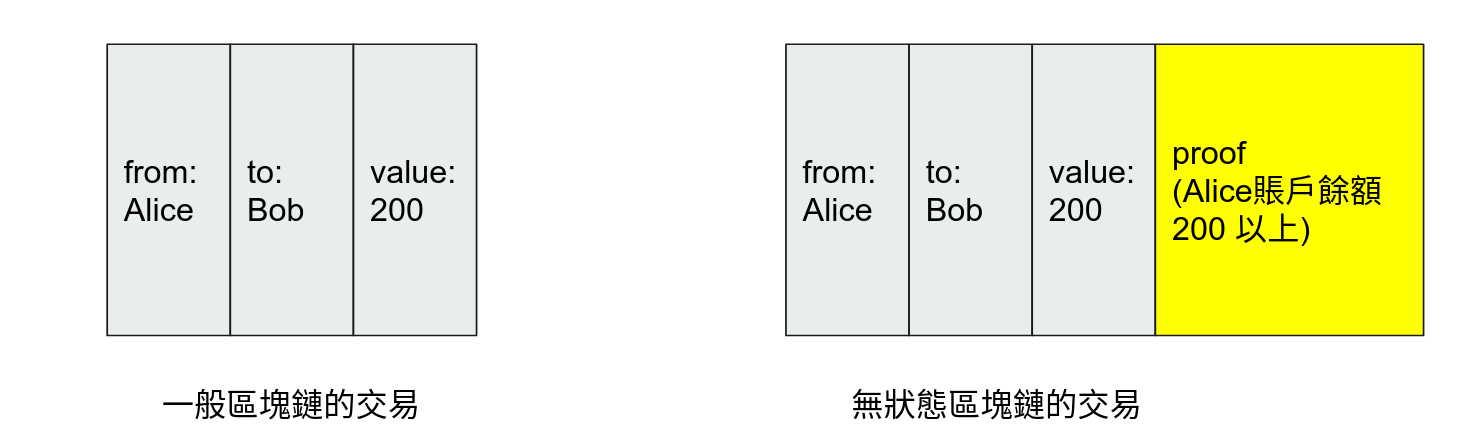
\includegraphics[width=\textwidth]{stateless-tx}
\caption{一般區塊鏈、無狀態區塊鏈交易比較}
\end{figure}

\subsection{vector commitment}

不僅僅上述的梅克爾樹變形能夠生成、更新摘要和證明,
可以做到這些功能的結構被稱為 vector commitment\cite{catalano2013vector}。

近年來, vector commitment 領域也持續出現不同針對無狀態區塊鏈的代數構造,
時空間複雜度或是常數往往更小。
有的能夠將多個證明打包以降低空間\cite{boneh2019batching},
有的則有同態加法的特性,使得製作交易證明時,付款人不用知道收款人的當前餘額\cite{chepurnoy2018edrax}。

\section{持久化資料結構}

如果一種資料結構在修改之後,能夠保留之前的版本,
就可以被稱為持久化資料結構\cite{driscoll1986making}(Persistent Data Structure),
與之相對的是暫時性資料結構(Ephemeral Data Structure)。

\subsection{路徑複製}
對於樹這種資料結構,可以利用路徑複製的技巧來將它變得持久化,
當樹中的一個節點被修改,就連帶修改指向它的父親節點,
如此一直遞迴往上修改到根節點,就可以得到一棵新版本的樹。

\begin{figure}
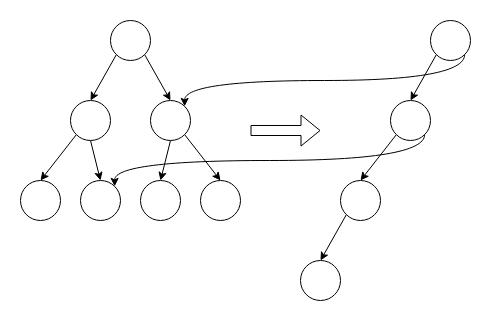
\includegraphics[width=\textwidth]{../images/路徑複製.png}
\caption{路徑複製}
\end{figure}

圖 2.2 是一個路徑複製的例子,可以從圖中看到,
只有被插入葉子的節點所在的分支被複製了一趟。